	\documentclass[10pt,twocolumn,letterpaper]{article}

\usepackage{cvpr}
\usepackage{times}
\usepackage{epsfig}
\usepackage{graphicx}
\usepackage{amsmath}
\usepackage{amssymb}
% Include other packages here, before hyperref.
\usepackage{hyperref}

\cvprfinalcopy % *** Uncomment this line for the final submission
\def\cvprPaperID{****} % *** Enter the CVPR Paper ID here
\def\httilde{\mbox{\tt\raisebox{-.5ex}{\symbol{126}}}}
% Pages are numbered in submission mode, and unnumbered in camera-ready
\ifcvprfinal\pagestyle{empty}\fi

% graphics pull from this folders
\graphicspath{{../figs/}}

\begin{document}
\title{Image Completion}

\author{Debora Sujono, Yue Tang \& Grace Yoo \\ 
University of Massachusetts Amherst \\ 
College of Information \& Computer Sciences \\
{\tt\small \{dsujono, gyoo, ytang\}@cs.umass.edu} \\
}

\maketitle

\section{Abstract} 
% no more than 300 words


\section{Introduction}
% Introduction: this section introduces your problem, and the overall plan for approaching your problem
Image completion, also called content-aware fill or inpainting, is a generative technique that can be used to fill missing areas of an image. The desired result is an image that a human would perceive as normal. These techniques are often implemented in photo-editing software to mend corrupted images.

\par We can conceptualize a photograph as a low-dimensional sample from a high-dimensional distribution, the original scene. The problem can be framed as learning these high-dimensional distributions such that we can generate a sample that approximates missing pixels. In our project, an incomplete image is treated as the lower-dimensional sample from the complete image. Contextual information from incomplete images, such as the values of pixels neighboring the missing content, can help inform the generative model. \\

%TODO n layer model
\par 
We will experiment with training generative models on observations of incomplete images $X$, and targets of original images $y$. The original images are from the CIFAR-10 dataset, and the incomplete versions have a square region removed from the center of the image. Using RNNs and CNNs, we will attempt to learn neuron weights to attempt modeling the area in $y$ corresponding to the missing region. We will randomly generate samples from these predictions, insert them into incomplete images, and use human judgment to determine if the predicted images are plausible. As a technical means of evaluation, we will use RMSE between $\hat y$ and $y$ to measure how different the images are. However, our main goal is to be able to complete images in general, which is why our hold out test set is comprised of incomplete images unknown to the model. For this reason, we don't consider RMSE to be the most important metric.\\

%TODO check if language in this paragraph sounds right...
%TODO more accurately describe the "simpler CNN" as nonlinear model bc of ReLU activation layers
Our simplest model is a n layer CNN with regression between $X$ and $y$, using RMSE loss. We also used RNNs designed to read pixels sequentially; one model used a pre-existing implementation of pixel RNN with sigmoidal output, the other model had 256-way categorical cross-entropy ("softmax loss"). We also used an adaptation of CNNs designed to emulate the sequential information feeding within a recurrent layer. We expected that the complex models, which sequentially approximate the joint distribution for each pixel, would outperform the simpler CNN using regression.\\

\section{Related Work} 
% This section discusses relevant literature for your project
Training a generative model can easily become intractable; we not only have to simulate high dimensional distributions, but also apply some kind of inference method to create a new sample. We decided to stick with feed-forward networks, where at test time the input is the incomplete image, and the output is the completed image. The following sections detail previous implementations of RNNs and CNNs adapted for sequentially scanning pixels in images.

\subsection{Pixel Recurrent Neural Networks}
The recurrent layers of an RNN have memory-like properties, which is why networks using specialized types of recurrent layers are called Long-Short Term Memory (LSTM) nets. These variants on recurrent layers were designed to ameliorate the exploding gradient sometimes experienced by vanilla recurrent layers. We think that the reason this happens in vanilla layers because feed forward networks with great depth generally have the potential for exploding gradients. At a high level, the way in which recurrent layers store previous information needs to be adjusted, in order to remember larger global patterns over iterations. LSTMs have a feature in recurrent layers, sometimes called a "gate", which determines if information from the previous cell will be fed forward, or forgotten. This gate is the hidden layer activation function, which for vanilla RNNs is often a sigmoid function. \cite{handwritingRNN}\\


% handwriting RNN paper
RNNs were used to generate convincing script from samples of handwriting. Previously, the handwriting generation problem posed a challenge because while the contextual information to generate individual letters may have been available from some models, many failed to learn higher-level sequences, such as stringing letters together. \cite{handwritingRNN} This seems particularly important in creating convincing samples of cursive handwriting styles. The cursive handwriting results from the network described by the Graves paper are pretty convincing. The inpainting problem is similar to handwriting generation in that it is important to preserve sequential features within and across layers.\\
%TODO what hyperparameter might this be? 

% main pixel RNN paper
\par
A study aimed to improve the efficiency of RNN architectures experimented with two different implementations of LSTMs that differed in the way they scanned across an image, collecting sequential data. The Row LSTM scans an image row by row, from top to bottom. The Diagonal Bidirectional LSTM (BiLSTM) simultaneously scans an image from the top left to the bottom right corner and from the top right to the bottom left corner. By skewing the inputs in a particular way, both diagonals are computed efficiently. The first step of the scanning is accomplished by a $1 \times 1$ convolution filter, which creates a tensor of $4h \times n \times n$ for $h$ hidden states and image with size $n \times n$. This can be thought of as a sliding mask. The second step is a column-wise sweep with a $2  \times  1$ convolution filter, which isn't masked. This is the part that facilitates recurrence within the layer. The authors noted that because the Diagonal LSTM already has a good receptive field with the second $2  \times  1$ kernel, increasing the size shouldn't improve the receptive field much. For both types of Pixel RNNs, van den Oord et al. suggest that networks can have up to 12 layers. A downside of LSTM layers is that you cannot parallelize the processes, as they must be computed sequentially. \cite{pixelRNN}

\subsection{Pixel Convolutional Neural Networks}
CNNs, despite lacking some kind of inherent sequential structure, can be modified to emulate the scanning accomplished by LSTM layers, without the cost associated with sequential computations. Using a convolutional filter to capture smaller areas of images and compute features within those receptive fields is a way to create a sliding mask over an image \cite{pixelRNN}. These computations can be parallelized, which makes the Pixel CNN worth exploring, since we weren't certain how long Pixel RNN would take to train. 

\section{Approach}
% Approach: This section details the framework of your project. Be specific, which means you might want to include equations, figures, plots, etc
Given an image with a square region of missing pixels, our goal is to fill in the missing pixels to create a cohesive image. We will use the CIFAR-10 dataset, which consists of $60,000$ images evenly distributed into 10 classes (airplane, automobile, bird, cat, deer, dog, frog, horse, ship, truck). Each $32 \times 32 \times 3$ pixel image is represented by the RGB color model. We will remove a square region of each image, and consider the original image to be the original distribution of $32 \times 32 \times 3 = 3,072$ dimensions. 

\par As our baseline, we will implement a convolutional neural net (CNN) with mean squared error (MSE) loss between incomplete and original images, to perform regression on the intensities of the missing pixels. From here, we will each investigate different generative modeling methods to improve the baseline score using the same evaluation.

\par After experimentation, we will optimize one or two models that we find most promising. We will use Root Mean Squared Error (RMSE) to compare models. The RMSE will give us an idea of how well our generated images compare to the originals; however, the problem is to generate any plausible images, so we will also randomly sample images for human judgment. We will ask judges to rate an image as "plausible" or "not plausible", and determine which models generate the most believable images. 

This is what our incomplete images look like after we mask part of it:

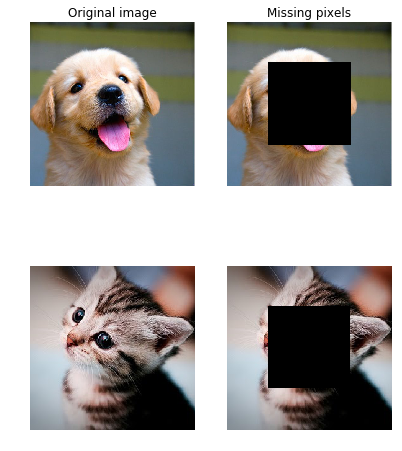
\includegraphics[width=1.0\linewidth]{img_sample.png}

Once we create a model that we can generate samples from, we'll use the model to create filled-in images $\hat{y}$.

Given the set of generated images $\hat{y}$. and corresponding original images $y$, we want to learn network parameters  $ \theta = [W_1, b_1, W_2, b_2, W_3, b_3]$ that minimize the MSE between generated and original images (or between incomplete and original images for the baseline case). 



Pixel RNNs approximate the joint distribution of pixels in the image by treating each pixel as a product of conditional distributions of all pixels previously seen in that layer.  This converts the problem into a sequence problem, and the task becomes to predict the next pixel given the previously generated ones \cite{pixelRNN}. 

Let $p(x)$ be the generated distribution for image $x$ with dimensions $n \times n$, represented as a row of length $n^2$. We approximate $p(x)$ by: \\
$p(x) = \prod_{i=1}^{n^2} p(x_i | x_1, ... , x_{i-1} )$




\section{Experiments} 
% This section begins with what kind of experiments you're doing, what kind of dataset(s) you're using, and what is the way you measure or evaluate your results. It then shows in details the results of your experiments. By details, we mean both quantitative evaluations (show numbers, figures, tables, etc) as well as qualitative results (show images, example results, etc).
In the following sections, we will outline the different training methods that we will implement. 

%TODO x layer
We compare the performance of a x layer CNN using regression with RMSE loss.


%Intermediate/Preliminary Results: State and evaluate your results upto the milestone
We have implemented a 3-layer CNN with regression using the following architecture: 
%$Convolutional \rightarrow ReLU \rightarrow 2x2 Max pooling \rightarrow affine \rightarrow ReLU \rightarrow affine \rightarrow MSE$

\begin{itemize}
\item Input: $32  \times  32  \times  3$ raw pixel values
\item Convolutional layer with $7  \times  7$ filter
\item ReLU activation
\item Pooling layer [2 x 2]
%: results [16 x 16 x 7]
\item Affine
\item ReLU activation
\item Affine
\item Output: sum previous layer, use RMSE loss function
\end{itemize}

This is not the final architecture we will use, we just decided to start with the architecture from Assignment 2 while we debug these first steps. 

We then trained the network for 1 epoch and achieved training RMSE of 120.323 and validation RMSE of 153.462. Our network is currently overfit, and since the values of the data range from 0.0 - 255.0, these RMSE values are quite high. We expect high RMSE because this is just the baseline network, but we are currently checking to make sure there aren't other issues causing such a high RMSE.

\section{Conclusion}
% Conclusion: What have you learned? Suggest future ideas.



%%%%% FUTURE IDEAS
%% data improvements
use domain knowledge by using same type of images (face, or categories of CIFAR)

%% high level modeling
evaluation: 
improve annotation collection, could possibly use annotations to label images for normalcy, and train on that
%TODO describe another metric that someone else has used to describe how normal an image seems to humans

one major limitation was not being able to tune efficiently over the full dataset. 
perhaps this is why simpler models perform well; we have the ability to tune them
combine speed of convolutions with recurrent structure to improve performance
%TODO describe specifically the structure of the multi-scale RNN 

major improvement would be to implement GANs and possibly DCGANs (efficiency?) given what we've learned about realistically training models using GPU instances, what challenges would we expect to face?



%% low level modeling
pixel rnn is too slow on its own, prediction for each pixel --> suggest ways to speed up


\begin{thebibliography}{1}
\bibitem{pixelRNN} Pixel Recurrent Neural Networks \url{https://arxiv.org/pdf/1601.06759v3}
\bibitem{handwritingRNN} Generating Sequences with Recurrent Neural Networks \url{https://arxiv.org/pdf/1308.0850v5.pdf}
\bibitem{pixelCNN} Conditional Image Generation with PixelCNN Decoders \url{https://arxiv.org/pdf/1606.05328v2.pdf}

\bibitem{GAN} Generative Adversarial Nets \url{http://papers.nips.cc/paper/5423-generative-adversarial-nets.pdf}
\bibitem{DCGAN} Unsupervised Representation Learning with Deep Convolutional Generative Adversarial Networks \url{https://arxiv.org/pdf/1511.06434v2}
\bibitem{inpaint} Semantic Image Inpainting with Perceptual and Contextual Losses \url{https://arxiv.org/pdf/1607.07539v2.pdf}
\end{thebibliography}


\end{document}
